\begin{usecase}{03}{Lista dei dispositivi}
\usecaseprimaryactors{Utente autenticato}
\usecasepre{L'utente ha accesso alla lista dei dispositivi collegati al proprio profilo.}
\usecasedesc{Viene visualizzata la lista dei dispositivi di cui l'utente può avere informazioni a riguardo.}
\usecasepost{Viene visualizzata la lista dei dispositivi di cui l'utente può avere informazioni a riguardo.}
\usecaseext{UC03.2}
\label{uc:UC03}
\end{usecase}

\begin{figure}[!h] 
    \centering 
    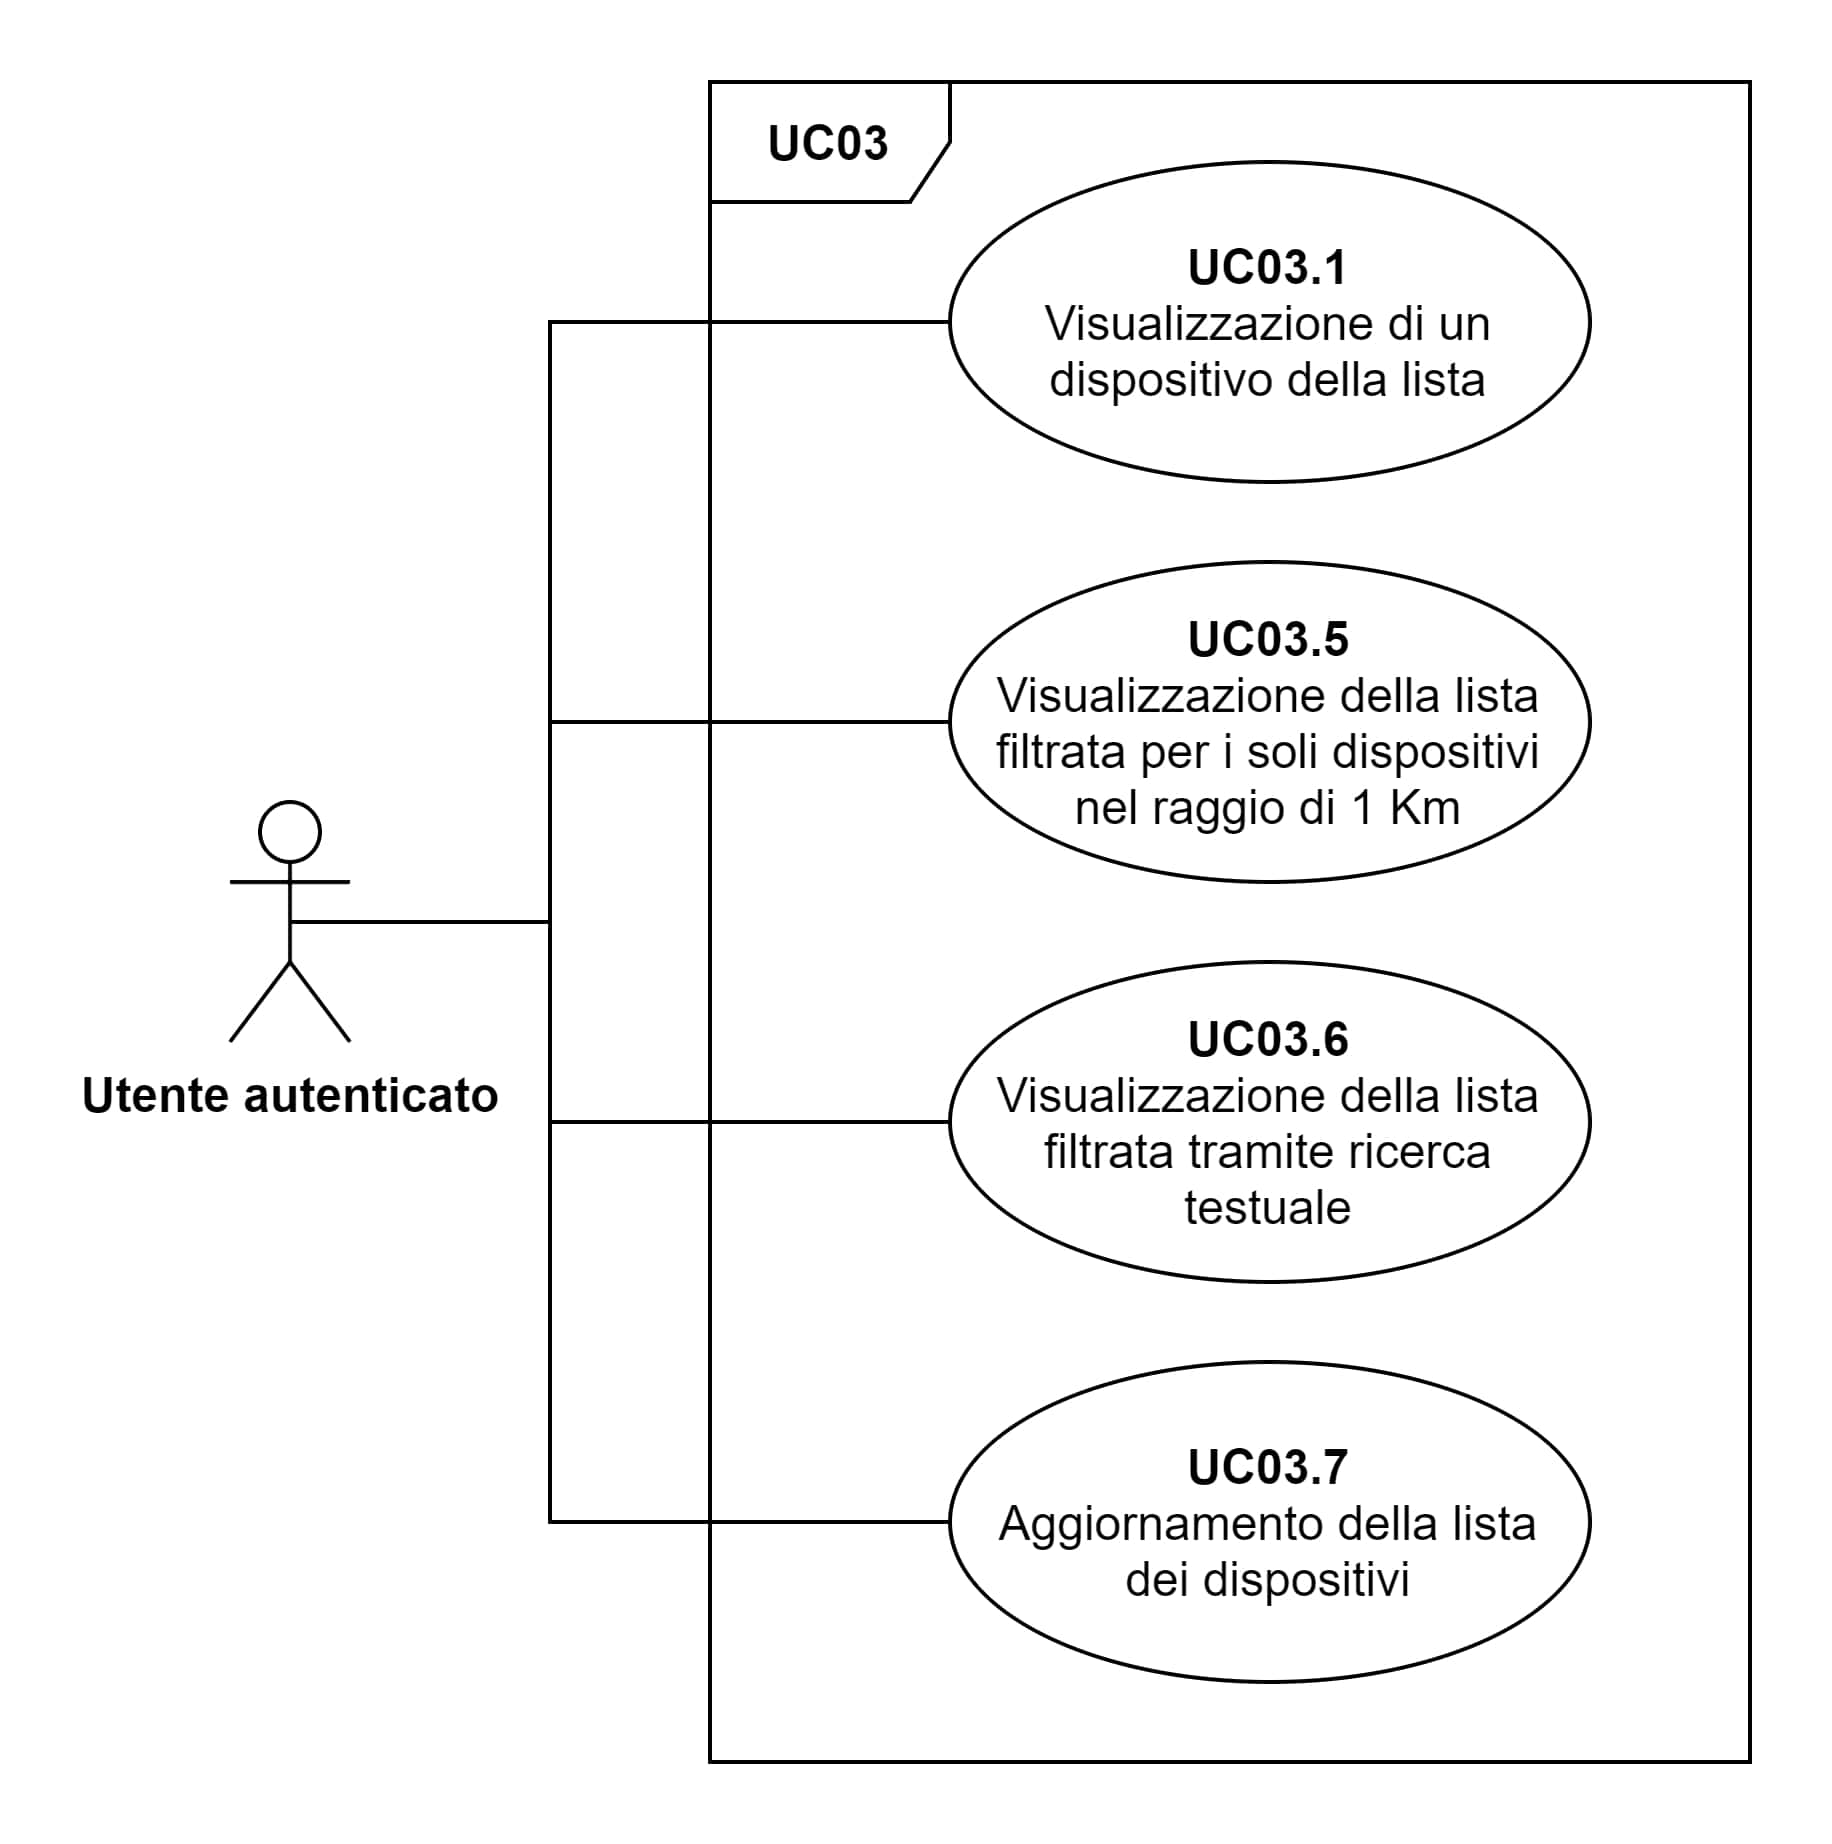
\includegraphics[width=1.0\columnwidth]{appendice-A/uc03} 
    \caption{SMacs - Sotto-casi d'uso di UC03 - Lista dei dispositivi}
\end{figure}

\begin{usecase}{03.1}{Visualizzazione di un dispositivo della lista}
\usecaseprimaryactors{Utente autenticato}
\usecasepre{L'utente sta visionando la lista dei dispositivi collegati al proprio profilo.}
\usecasedesc{Viene visualizzato un dispositivo della lista dei dispositivi collegati al profilo dell'utente, mostrandone un'icona rappresentativa e un dettaglio compatto che comprende il codice, il nome, lo stato attuale e il livello massimo di segnalazione attuale. Inoltre, viene mostrata la data di ultimo aggiornamento.}
\usecasepost{Viene visualizzato un dispositivo della lista dei dispositivi collegati al profilo dell'utente, mostrandone un dettaglio compatto.}
\label{uc:UC03-1}
\end{usecase}

\begin{usecase}{03.2}{Visualizzazione di una segnalazione quando la lista dei dispositivi è vuota}
\usecaseprimaryactors{Utente autenticato}
\usecasepre{L'utente sta visionando la lista dei dispositivi collegati al proprio profilo ma è vuota.}
\usecasedesc{L'utente sta visionando la lista dei dispositivi collegati al proprio profilo ma è vuota, quindi viene avvisato mediante un messaggio,}
\usecasepost{Viene visualizzato un messaggio che avvisa l'utente che la lista è vuota.}
\label{uc:UC03-2}
\end{usecase}

\begin{usecase}{03.3}{Visualizzazione della lista in ordine alfabetico}
\usecaseprimaryactors{Utente autenticato}
\usecasepre{L'utente sta visionando la lista dei dispositivi collegati al proprio profilo.}
\usecasedesc{Viene visualizzata la lista dei dispositivi di cui l'utente può avere informazioni a riguardo in ordine alfabetico (corrisponde all'opzione di default).}
\usecasepost{Viene visualizzata la lista dei dispositivi di cui l'utente può avere informazioni a riguardo in ordine alfabetico.}
\usecasegen{UC03}
\label{uc:UC03-3}
\end{usecase}

\begin{usecase}{03.4}{Visualizzazione della lista dei soli dispositivi con segnalazioni}
\usecaseprimaryactors{Utente autenticato}
\usecasepre{L'utente sta visionando la lista dei dispositivi collegati al proprio profilo.}
\usecasedesc{Viene visualizzata la lista dei dispositivi con segnalazioni (di malfunzionamento) di cui l'utente può avere informazioni a riguardo.}
\usecasepost{Viene visualizzata la lista dei dispositivi con segnalazioni (di malfunzionamento) di cui l'utente può avere informazioni a riguardo.}
\usecasegen{UC03}
\label{uc:UC03-4}
\end{usecase}

\begin{usecase}{03.5}{Visualizzazione della lista filtrata per i soli dispositivi nel raggio di 1 Km}
\usecaseprimaryactors{Utente autenticato}
\usecasepre{L'utente sta visionando la lista dei dispositivi collegati al proprio profilo.}
\usecasedesc{Viene visualizzata la lista dei dispositivi entro il raggio di 1 Km dalla posizione geografica attuale dell'utente di cui l'utente può avere informazioni a riguardo.}
\usecasepost{Viene visualizzata la lista dei dispositivi entro il raggio di 1 Km dalla posizione geografica attuale dell'utente di cui l'utente può avere informazioni a riguardo.}
\label{uc:UC03-5}
\end{usecase}

\begin{usecase}{03.6}{Visualizzazione della lista filtrata tramite ricerca testuale}
\usecaseprimaryactors{Utente autenticato}
\usecasepre{L'utente sta visionando la lista dei dispositivi collegati al proprio profilo.}
\usecasedesc{Viene visualizzata la lista dei dispositivi in base alla ricerca inoltrata di cui l'utente può avere informazioni a riguardo.}
\usecasepost{Viene visualizzata la lista dei dispositivi in base alla ricerca inoltrata di cui l'utente può avere informazioni a riguardo.}
\label{uc:UC03-6}
\end{usecase}

\begin{usecase}{03.7}{Aggiornamento della lista dei dispositivi}
\usecaseprimaryactors{Utente autenticato}
\usecasepre{L'utente sta visionando la lista dei dispositivi collegati al proprio profilo.}
\usecasedesc{L'utente seleziona la funzionalità di aggiornamento e viene aggiornata la lista dei dispositivi di cui l'utente può avere informazioni a riguardo ottenendone una nuova copia dal sistema.}
\usecasepost{L'utente seleziona la funzionalità di aggiornamento e viene aggiornata la lista dei dispositivi di cui l'utente può avere informazioni a riguardo ottenendone una nuova copia dal sistema.}
\label{uc:UC03-7}
\end{usecase}